%
%Не забыть:
%--------------------------------------
%Вставить колонтитулы, поменять название на титульнике



%--------------------------------------

\documentclass[a4paper, 12pt]{article} 

%--------------------------------------
%Russian-specific packages
%--------------------------------------
%\usepackage[warn]{mathtext}
\usepackage[T2A]{fontenc}
\usepackage[utf8]{inputenc}
\usepackage[english]{babel}
\usepackage[intlimits]{amsmath}
\usepackage{esint}
%--------------------------------------
%Hyphenation rules
%--------------------------------------
\usepackage{hyphenat}
\hyphenation{ма-те-ма-ти-ка вос-ста-нав-ли-вать}
%--------------------------------------
%Packages
%--------------------------------------
\usepackage{amsmath}
\usepackage{amssymb}
\usepackage{amsfonts}
\usepackage{amsthm}
\usepackage{latexsym}
\usepackage{mathtools}
\usepackage{etoolbox}%Булевые операторы
\usepackage{extsizes}%Выставление произвольного шрифта в \documentclass
\usepackage{geometry}%Разметка листа
\usepackage{indentfirst}
\usepackage{wrapfig}%Создание обтекаемых текстом объектов
\usepackage{fancyhdr}%Создание колонтитулов
\usepackage{setspace}%Настройка интерлиньяжа
\usepackage{lastpage}%Вывод номера последней страницы в документе, \lastpage
\usepackage{soul}%Изменение параметров начертания
\usepackage{hyperref}%Две строчки с настройкой гиперссылок внутри получаеммого
\usepackage[usenames,dvipsnames,svgnames,table,rgb]{xcolor}% pdf-документа
\usepackage{multicol}%Позволяет писать текст в несколько колонок
\usepackage{cite}%Работа с библиографией
\usepackage{subfigure}% Человеческая вставка нескольких картинок
\usepackage{tikz}%Рисование рисунков
\usetikzlibrary{circuits} % подключаем библиотеки, содержащие
\usetikzlibrary{circuits.ee} % УГО для схем
\usetikzlibrary{circuits.ee.IEC}
\usetikzlibrary{arrows} % подключаем библиотеки со стрелками
\usetikzlibrary{patterns} % и со штриховкой
\usepackage{float}% Возможность ставить H в положениях картинки
% Для картинок Моти
\usepackage{misccorr}
\usepackage{lscape}
\usepackage{cmap}
\usepackage{bm}
\newtheorem{definition}{Definition}



\usepackage{graphicx,xcolor}
\graphicspath{{Pictures/}}
\DeclareGraphicsExtensions{.pdf,.png,.jpg}

%----------------------------------------
%Список окружений
%----------------------------------------
\newenvironment {theor}[2]
{\smallskip \par \textbf{#1.} \textit{#2}  \par $\blacktriangleleft$}
{\flushright{$\blacktriangleright$} \medskip \par} %лемма/теорема с доказательством
\newenvironment {proofn}
{\par $\blacktriangleleft$}
{$\blacktriangleright$ \par} %доказательство
%----------------------------------------
%Список команд
%----------------------------------------
\newcommand{\grad}
{\mathop{\mathrm{grad}}\nolimits\,} %градиент

\newcommand{\diver}
{\mathop{\mathrm{div}}\nolimits\,} %дивергенция

\newcommand{\rot}
{\ensuremath{\mathrm{rot}}\,}

\newcommand{\Def}[1]
{\underline{\textbf{#1}}} %определение

\newcommand{\RN}[1]
{\MakeUppercase{\romannumeral #1}} %римские цифры

\newcommand {\theornp}[2]
{\textbf{#1.} \textit{ #2} \par} %Написание леммы/теоремы без доказательства

\newcommand{\qrq}
{\ensuremath{\quad \Rightarrow \quad}} %Человеческий знак следствия

\newcommand{\const}{\text{const}} % Написание const в формулах

\newcommand{\qlrq}
{\ensuremath{\quad \Leftrightarrow \quad}} %Человеческий знак равносильности

\renewcommand{\phi}{\varphi} %Нормальный знак фи

\renewcommand{\epsilon}{\varepsilon}

\newcommand{\me}
{\ensuremath{\mathbb{E}}}

\newcommand{\md}
{\ensuremath{\mathbb{D}}}



%\renewcommand{\vec}{\overline}




%----------------------------------------
%Разметка листа
%----------------------------------------
\geometry{top = 3cm}
\geometry{bottom = 2cm}
\geometry{left = 1.5cm}
\geometry{right = 1.5cm}
%----------------------------------------
%Колонтитулы
%----------------------------------------
\pagestyle{fancy}%Создание колонтитулов
\fancyhead{}
%\fancyfoot{}
\fancyhead[R]{\textsc{Diffraction}}%Вставить колонтитул сюда
%----------------------------------------
%Интерлиньяж (расстояния между строчками)
%----------------------------------------
%\onehalfspacing -- интерлиньяж 1.5
%\doublespacing -- интерлиньяж 2
%----------------------------------------
%Настройка гиперссылок
%----------------------------------------
\hypersetup{				% Гиперссылки
	unicode=true,           % русские буквы в раздела PDF
	pdftitle={Заголовок},   % Заголовок
	pdfauthor={Author},      % Автор
	pdfsubject={Subject},      % Тема
	pdfcreator={Creatir}, % Создатель
	pdfproducer={Producer}, % Производитель
	pdfkeywords={keyword1} {key2} {key3}, % Ключевые слова
	colorlinks=false,       	% false: ссылки в рамках; true: цветные ссылки
	linkcolor=blue,          % внутренние ссылки
	citecolor=blue,        % на библиографию
	filecolor=magenta,      % на файлы
	urlcolor=blue           % на URL
}
%----------------------------------------
%Работа с библиографией 
%----------------------------------------
\renewcommand{\refname}{Список литературы}%Изменение названия списка литературы для article
%\renewcommand{\bibname}{Список литературы}%Изменение названия списка литературы для book и report
%----------------------------------------
\begin{document}
	\begin{titlepage}
		\begin{center}
			$$$$
			$$$$
			$$$$
			$$$$
			{\Large{NATIONAL RESEARCH UNIVERSITY}}\\
			\vspace{0.1cm}
			{\Large{HIGHER SCHOOL OF ECONOMICS}}\\
			\vspace{0.25cm}
			{\large{Faculty of Physics}}\\
			\vspace{5.5cm}
			{\Huge\textbf{{Report}}}\\%Общее название
			\vspace{1cm}
			{\LARGE{<<Diffraction>>}}\\%Точное название
			\vspace{1cm}
			{\large{M. I. Blumenau}}\\%Me
			\vspace{2cm}
			\vfill
			
\includegraphics[width = 0.2\textwidth]{HSElogo}\\
			\vfill
			Moscow\\
			2021
		\end{center}
	\end{titlepage}
	
	\tableofcontents
	\newpage
	\addcontentsline{toc}{section}{Introduction}
	\section*{Introduction}
	This report represents an assembly of an installation for observing diffraction on a reflecting diffraction grating. We studied the diffraction pattern for different gratings at different angles of incidence of light, determined the positions of the maxima. For each grid, we determined the number of strokes per unit length. Using a photodiode power meter, we measured the light intensity in maxima for the grating with which the greatest number of maxima was observed. After processing the obtained dependence, we determined the angle of the lattice bevel $\gamma$.
	\addcontentsline{toc}{section}{Theoretical information}
	\section*{Theoretical information}
	\addcontentsline{toc}{subsection}{Single-slit diffraction}
	\subsection*{Single-slit diffraction}
	Let the edges of the gap be located at $x = \pm b / 2$, where $b$ is the width of the gap. A plane monochromatic wave with a wave vector $k$ at an angle $\theta_i$ to the normal vector to the lattice falls on the slit.
	\begin{figure}[H]
		\centering
		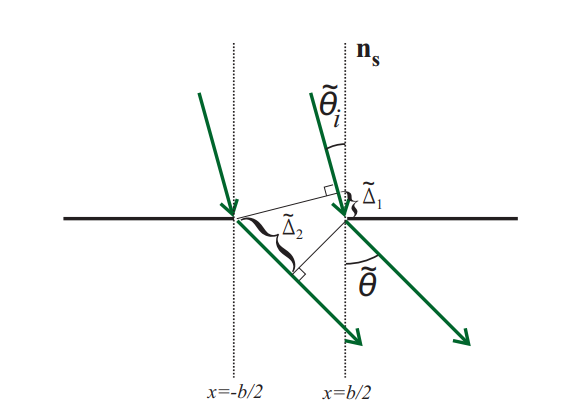
\includegraphics[width=0.85\linewidth]{diff1.png}
		\caption{Fraunhofer diffraction on the slit.}
		\label{fig:1}
	\end{figure}
	The phase difference between the waves emitted from the coordinate $x = 0$ and $x$ is equal to $ \delta_1 = - k x (\sin {\theta} + sin {\theta_i})$. We obtain:
	\begin{equation}
		E(\theta) \propto \int_{b/2}^{b/2}{\exp(-i \delta_1(x))dx} \propto \int_{b/2}^{b/2}{\exp(-i k x (\sin{\theta} + \sin{\theta_i})) dx}
	\end{equation}
	\begin{equation}
		E(\theta) \propto \frac{\sin(k b / 2 (\sin{\theta} + \sin{\theta_i})}{k b / 2 (\sin{\theta} + \sin{\theta_i}}
	\end{equation}
	\addcontentsline{toc}{subsection}{Diffraction on a lattice with $N$ slits}
	\subsection*{Diffraction on a lattice with $N$ slits}
	The path difference between the secondary waves formed by adjacent slits is $ \ delta = d k (\sin{\theta} + \ sin{\theta_i})$, in addition, the field emitted by the slot with the number $n$ is $ E_n = E_1 \exp(-i \delta n)$. Hence the resulting field:
	\begin{equation}
		E = E_1 * \sum_{0}^{N-1} \exp(-i \delta n) = E_1 \exp(i\delta(N/2 - 1)) \frac{\sin(N \delta /2)}{\sin(\delta /2)}
	\end{equation}
	From here we can obtain the intensity:
	\begin{equation}
		I \propto E^2 \propto (\frac{\sin(k b / 2 (\sin{\theta} + \sin{\theta_i}))}{k b / 2 (\sin{\theta} + \sin{\theta_i})})^2 \cdot (\frac{\sin(N k d / 2 (\sin{\theta} + sin{\theta_i}))}{\sin(k d / 2 (\sin{\theta} + sin{\theta_i}))})^2
	\end{equation}
	The right multiplier is responsible for the position of the observed maxima, it also gives us the following condition:
	\begin{equation}
		d(\sin{\theta} + \sin{\theta_i}) = m \lambda,
	\end{equation}
	where $m$ is an integer called the order of the maximum.
	\addcontentsline{toc}{subsection}{Diffraction on a concentrating reflecting array}
	\subsection*{Diffraction on a concentrating reflecting array}
	Because of the geometry of the concentrating reflecting grid, the multiplier $E_1(\theta)$ will change, while the second multiplier will remain the same.
	\begin{equation}
		I \propto E^2 \propto (\frac{\sin(k b / 2 (\sin(\theta - \gamma) + \sin(\theta_i - \gamma)))}{k b / 2 (\sin(\theta - \gamma) + \sin(\theta_i - \gamma))})^2 \cdot  (\frac{\sin(N k d / 2 (\sin{\theta} + sin{\theta_i}))}{\sin(k d / 2 (\sin{\theta} + sin{\theta_i}))})^2
	\end{equation}
	
	\begin{figure}[H]
		\centering
		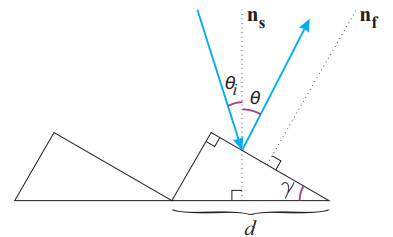
\includegraphics[width=0.85\linewidth]{diff2.png}
		\caption{Diffraction on a concentrating reflecting array.}
		\label{fig:2}
	\end{figure}
	
	Here we will be interested in the first, changed multiplier, which is the curve that envelopes the intensity.
	
	The angle at which the maximum intensity is observed corresponds to the mirror reflection of the incident light, is called the angle of brightness, and is defined by the following expression:
	\begin{equation}
		\phi_B = 2\gamma - \theta_i
	\end{equation}
	We can also calculate the amount of slits per unit length using
	\begin{equation}
		N_{slit} = \alpha / (\lambda \cdot 10^{-6})
	\end{equation}
	\addcontentsline{toc}{section}{Equipment and methods}
	\section*{Equipment and methods}
	We used a laser with a wavelength of 520 nm, reflecting diffraction gratings with different lattice constants, a tape measure fixed on the wall, a ruler, and a light intensity analyzer.
	
	The results were collected by hand and later processed with Python. Schematic diagram of the installation attached below:
	\begin{figure}[H]
		\centering
		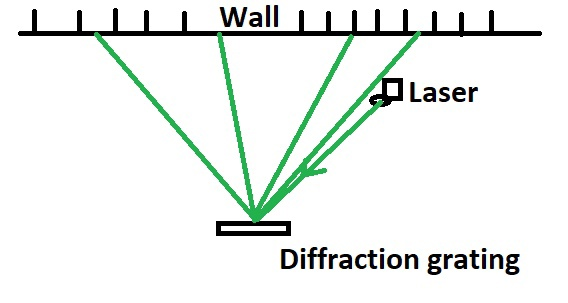
\includegraphics[width=0.85\linewidth]{sch1.jpg}
		\caption{Installation diagram.}
		\label{fig:3}
	\end{figure}
	
	Source code link:
	\newline
	\href{https://github.com/burunduk387/HSE-FF/tree/main/LabOptics/Diffraction}{https://github.com/burunduk387/HSE-FF/tree/main/LabOptics/Diffraction}
	\addcontentsline{toc}{section}{Experimental results}
	\section*{Experimental results}
	We fixed each diffraction grating in front of the screen, which was a wall with a fixed tape measure for measuring the coordinates of the beams on the screen. We moved the laser to change the angles of incidence of the beam on the grid and recorded the results. We repeated this experiment for all three gratings. Distance between the wall and the diffraction gratings remained the same throughout all experiments and was $L = 130$ cm. Y-coordinate distance between the diffraction grating and the laser also remained the same and was $a = 51.5$ cm. Different angles were achived by moving the laser X-wise. Raw data for angles different from $\theta_{i} = 0$ are available in the GitHub repository in order not to overload this report with information.
	\addcontentsline{toc}{subsection}{The first diffraction grating}
	\subsection*{The first diffraction grating}
	The results are represented in a table below.
	\begin{table}[H]
		\centering
		\caption{Table with raw data for $\theta_{i} = 0$.}
		\begin{tabular}[t]{lcc}
			\hline
			Order of the maximum&Coordinate of the maximum, cm\\
			\hline
			-1&77\\
			0&173.5\\
			1&282.5\\
			\hline
		\end{tabular}
	\end{table}
	\begin{figure}[H]
		\centering
		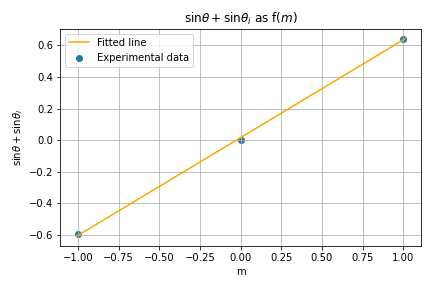
\includegraphics[width=0.75\linewidth]{1200.png}
		\caption{}
		\label{fig:1200}
	\end{figure}
	Unfortunately, our measuring tape was not long enough, so we were able to make only one measurement. After fitting a line, we get its coeffitiets. We obtain $N_{slit} = 1190 \pm 7  mm^{-1}$.
	\addcontentsline{toc}{subsection}{The second diffraction grating}
	\subsection*{The second diffraction grating}
	The results are represented in a table below.
	\begin{table}[H]
		\centering
		\caption{Table with raw data for $\theta_{i} = 0$.}
		\begin{tabular}[t]{lcc}
			\hline
			Order of the maximum&Coordinate of the maximum, cm\\
			\hline
			-2&55\\
			-1&124\\
			0&166\\
			1&207\\
			2&266\\
			\hline
		\end{tabular}
	\end{table}
	\begin{figure}[H]
		\centering
		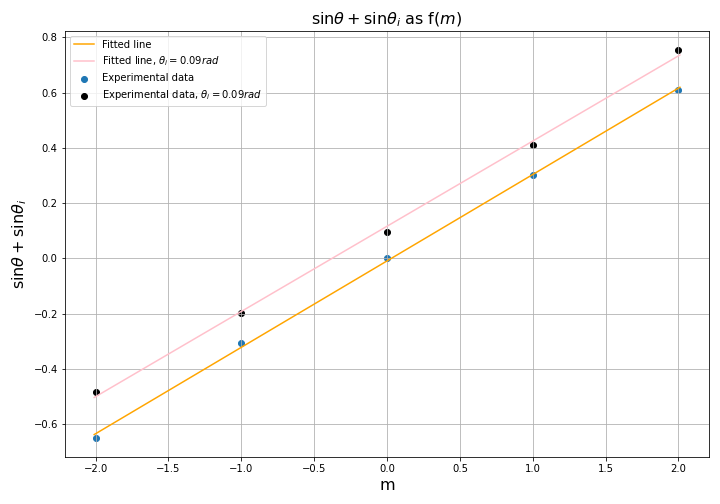
\includegraphics[width=0.75\linewidth]{600.png}
		\caption{}
		\label{fig:600}
	\end{figure}
	After fitting lines, we get their coeffitiets. We obtain $N_{slit} = 597 \pm 8 mm^{-1}$.
	\addcontentsline{toc}{subsection}{The third diffraction grating}
	\subsection*{The third diffraction grating}
	The results are represented in a table below. 
	\begin{table}[H]
		\centering
		\caption{Table with raw data for $\theta_{i} = 0$.}
		\begin{tabular}[t]{lcc}
			\hline
			Order of the maximum&Coordinate of the maximum, cm\\
			\hline
			-2&118\\
			-1&141\\
			0&161\\
			1&181\\
			2&202\\
			\hline
		\end{tabular}
	\end{table}
	\begin{figure}[H]
		\centering
		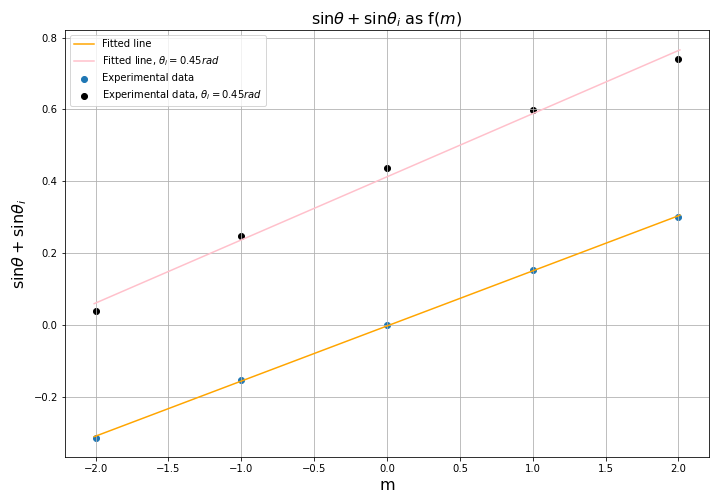
\includegraphics[width=0.75\linewidth]{300.png}
		\caption{}
		\label{fig:300}
	\end{figure}
	After fitting lines, we get their coeffitiets. We obtain $N_{slit} = 316 \pm 3 mm^{-1}$.
	\addcontentsline{toc}{subsection}{The second experiment}
	\subsection*{The second experiment}
	For the third grating, we attempted to find $\gamma$ using a light intensity analyzer. The results we got and the theoretical curve that was fitted are shown below.
	\begin{figure}[H]
		\centering
		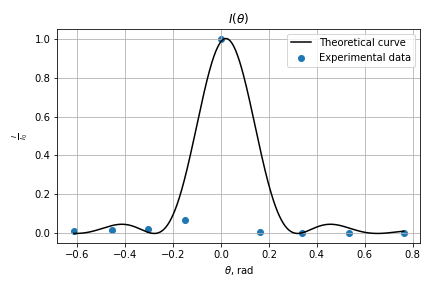
\includegraphics[width=0.85\linewidth]{gamma.png}
		\caption{}
		\label{fig:10}
	\end{figure}
	We got $\gamma = 0.012 \pm 0.005$ rad.
	\addcontentsline{toc}{section}{Conclusion}
	\section*{Conclusion}
	We attempted to calculate the amount of splits per unit length for three diffraction graters. For the third one we also tried to find its bevel angle. The results are:
	\begin{itemize}
		\item $N_{slit1} = 1190 \pm 7 mm^{-1}$
		\item $N_{slit2} = 597 \pm 8 mm^{-1}$
		\item $N_{slit3} = 316 \pm 3 mm^{-1}$.
		\item $\gamma = 0.012 \pm 0.005$ rad
	\end{itemize}
	\addcontentsline{toc}{section}{References}
	\begin{thebibliography}{9}
		\bibitem{bel} 
		Diffraction.
		Guidelines for the Optics Workshop, 2021.
	\end{thebibliography}
\end{document}
